%----------- Necessary Style Preamble -----------%

\documentclass[mathserif, 10pt]{beamer} %

\usepackage[framesassubsections]{beamerprosper}
\usepackage{beamerthemesplit} % Activate for custom appearance
\usepackage[english]{babel}
\usepackage[latin1]{inputenc}
\usepackage{amsmath, hyperref, subfigure, multirow, rotating}
\usepackage{epstopdf}
\usepackage{verbatim}
\usepackage{listings}
\usepackage{color}
\usepackage{esint}
\usepackage{mathrsfs}
\usepackage{multicol}
\usepackage{tikz}
\def\checkmark{\tikz\fill[scale=0.4](0,.35) -- (.25,0) -- (1,.7) -- (.25,.15) -- cycle;}

%\usepackage{enumitem}

\usetheme{Frankfurt}
\usecolortheme{default}
\usecolortheme[rgb={0.1,0.4,0.0}]{structure} % CSU color style
%\usecolortheme[rgb={0.541,0.149,0.196}]{structure} % BME color style

\setbeamersize{text margin left=0.5cm}
\setbeamersize{text margin right=0.5cm}

\setbeamercovered{transparent}

\usepackage{remreset}
\makeatletter
\@removefromreset{subsection}{section}
\makeatother
\setcounter{subsection}{1}

\makeatletter
\newcommand\xleftrightarrow[2][]{\ext@arrow 0099{\longleftrightarrowfill@}{#1}{#2}}
\def\longleftrightarrowfill@{\arrowfill@\leftarrow\relbar\rightarrow}
\makeatother


\newcommand\Wider[2][3em]{%
\makebox[\linewidth][c]{%
  \begin{minipage}{\dimexpr\textwidth+#1\relax}
  \raggedright#2
  \end{minipage}%
  }%
}

%----------- Math Definitions -----------%

\definecolor{Blue}{rgb}{0,0,1}
\def\ci{\perp\!\!\!\perp}
\def\a{\mathbf{a}}
\def\d{\mathbf{d}}
\def\e{\mathbf{e}}
\def\f{\mathbf{f}}
\def\g{\mathbf{g}}
\def\b{\mathbf{b}}
\def\q{\mathbf{q}}
\def\v{\mathbf{v}}
\def\x{\mathbf{x}}
\def\y{\mathbf{y}}
\def\u{\mathbf{u}}
%\def\z{\mathbf{\mathfrak{z}}}
\def\z{\mathbf{z}}
\def\D{\mathbf{D}}
\def\S{\mathbf{S}}
\def\X{\mathbf{X}}
\def\Z{\mathbf{Z}}
\def\1{\raisebox{.5pt}{\textcircled{\raisebox{-.9pt} {1}}}}
\def\2{\raisebox{.5pt}{\textcircled{\raisebox{-.9pt} {2}}}}
\def\3{\raisebox{.5pt}{\textcircled{\raisebox{-.9pt} {3}}}}
\def\4{\raisebox{.5pt}{\textcircled{\raisebox{-.9pt} {4}}}}
\def\5{\raisebox{.5pt}{\textcircled{\raisebox{-.9pt} {5}}}}
\def\6{\raisebox{.5pt}{\textcircled{\raisebox{-.9pt} {6}}}}
\def\balph{\boldsymbol\alpha}
\def\bmu{\boldsymbol\mu}
\def\btheta{\boldsymbol\theta}
\def\bomega{\boldsymbol\omega}
\def\bDelta{\boldsymbol\Delta}

%----------- Title Page Parameters -----------%
\title[Digital Control \& Digital Filters]{Digital Controls \& Digital Filters \\ Lectures 19 \& 20}
\author[M.R. Azimi]{M.R. Azimi, Professor}
\institute[CSU-ECE]{Department of Electrical and Computer Engineering \\ Colorado State University}
\date{Spring 2017}

\logo{
\includegraphics[height=0.5cm]{csu-logo.png}}

\newcommand{\unt}[1]{ \mathrm{\ #1}}

\begin{document}

%----------- slide --------------------------------------------------%

\frame{\titlepage}




\section{Stability Analysis of Digital Control Systems}
%----------- slide --------------------------------------------------%
\frame
{
%\vspace{-.2in}
\normalsize
%\renewcommand{\theenumi}{\alph{enumi}}
\frametitle{Stability Analysis (Chapter 7)}
\vspace{-.5in}
\textcolor{blue}{Definition 1: Bounded Input, Bounded Output (BIBO) Stability}\\
An LTI system is BIBO stable iff a bounded input yields a bounded output (for any IC), i.e. \\ \vspace{0.07in}
If $|x(n)|<M<\infty \implies|y(n)|<N<\infty$\\ \vspace{0.1in}
\textcolor{red}{Theorem 1:}\\
The necessary and sufficient condition for BIBO stability \\
is that the impulse response $h(n)$ is absolutely summable. \\ \vspace{0.07in}
$\sum\limits_{n=0}^{\infty} |h(n)| <P<\infty$\\ \vspace{0.1in}
\textcolor{blue}{Definition 2: Asymptotic Stability}\\
Consider autonomous (no input) LTI system:\\
$\x(n+1) = A\x(n)$\\
System is asymptotically stable iff for any IC $\x(0)$ such that \\  \vspace{0.07in}
$||\x(0)||<\delta \implies \lim\limits_{n\to\infty} ||\x(n)|| = 0$ \\ \vspace{0.05in}
where $||\x||$ represents the Euclidean norm of vector $\x$.

\vspace{-2in}
\hspace{3.25in}
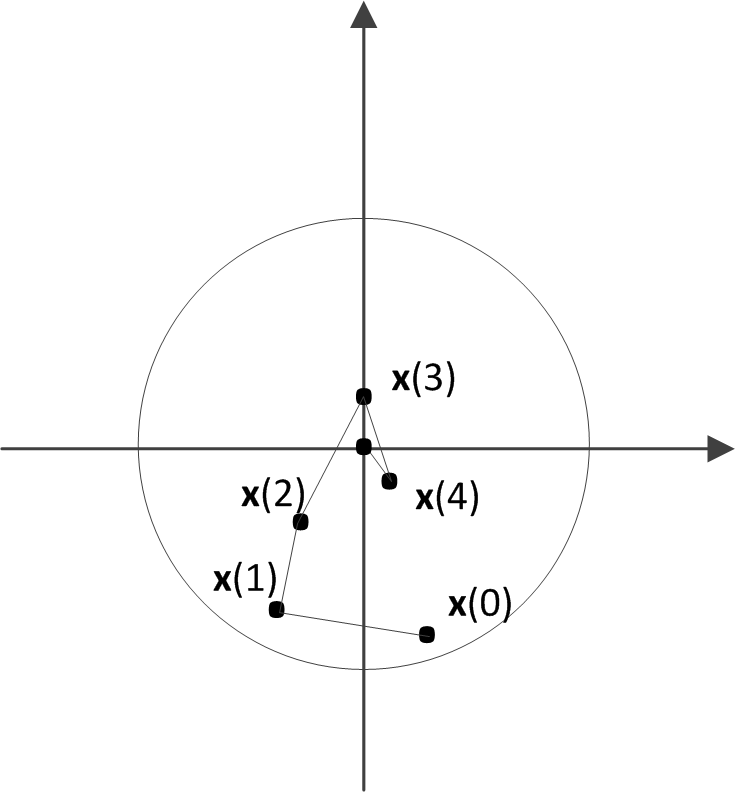
\includegraphics[width=.275\linewidth]{./Figures/assy_stable.png}
}

%----------- slide --------------------------------------------------%
\frame
{
%\vspace{-.2in}
\normalsize
%\renewcommand{\theenumi}{\alph{enumi}}
\frametitle{Stability Analysis-Cont.}

\textcolor{red}{Theorem 2:}\\
A discrete-time LTI system given before, is asymptotically stable iff all the eigenvalues of matrix $A$ (poles of the system)
lie strictly inside the unit circle. \\ \vspace{0.1in}

\textcolor{red}{Theorem 3:}\\
Asymptotic stability implies BIBO stability and vice versa. \\ \vspace{0.15in}


\textcolor{red}{Example:}  Consider the following LTI system \\ \vspace{0.07in}
$\x(n+1) = \left[
\begin{array}{cc}
	0&1\\
	-1&0
\end{array}\right] \x(n)+\left[
\begin{array}{c}
	1\\
	0
\end{array}\right] u(n)$\\
$y(n) = \left[
\begin{array}{cc}
	1&0
\end{array} \right] \x(n)$\\
The roots of CE or eigenvalues of matrix $A$ are obtained by solving,
$\varrho(z) =|zI-A| = \left|
\begin{array}{cc}
 	z&-1\\
	1&z
\end{array} \right| = (z^2+1)=0 \implies z_{1,2} = \pm j = e^{\pm j\pi/2}$\\

i.e. roots on the unit circle and hence not asymptotically stable.  \\
On the other hand, we can test for BIBO stability by finding $h(n)$ and checking absolute summable requirement.

}

%----------- slide --------------------------------------------------%
\frame
{
%\vspace{-.2in}
\normalsize
%\renewcommand{\theenumi}{\alph{enumi}}
\frametitle{Stability Analysis-Cont.}

State transition matrix, \\ \vspace{0.05in}
$A^n = \phi(n) = \mathcal{Z}^{-1}\left[( zI-A)^{-1}z\right]$\\ \vspace{0.05in}
$(zI-A)^{-1} = \frac{ \left[
\begin{array}{cc}
	z&1\\
	-1&z
\end{array} \right]}{z^2+1}$ \\
$A^n = \mathcal{Z}^{-1} \left[
\begin{array}{cc}
	\frac{z^2}{z^2+1}&\frac{z}{z^2+1}\\
	\frac{-z}{z^2+1}&\frac{z^2}{z^2+1}
\end{array}\right] = \left[
\begin{array}{cc}
	\cos{\frac{n\pi}{2}} & \sin{\frac{n\pi}{2}}\\
	-\sin{\frac{n\pi}{2}}&\cos{\frac{n\pi}{2}}
\end{array} \right]$\\ \vspace{0.05in}

Then the impulse response, $h(n) = C A^{n-1} B$,  becomes, \\ \vspace{0.05in}
$h(n) = \left[
\begin{array}{cc}
	1&0
\end{array} \right] \left[
\begin{array}{cc}
	\cos{\frac{(n-1)\pi}{2}} & \sin{\frac{(n-1)\pi}{2}}\\
	-\sin{\frac{(n-1)\pi}{2}}&\cos{\frac{(n-1)\pi}{2}}
\end{array} \right] \left[
\begin{array}{c}
	1\\
	0
\end{array} \right] = \cos{\frac{(n-1)\pi}{2}}$\\
$\sum\limits_{n=0}^\infty |h(n)| = \sum\limits_{n=0}^\infty |\cos{\frac{(n-1)\pi}{2}}| \to \infty$\\ \vspace{0.05in}
i.e.  not BIBO stable.

}

%----------- slide --------------------------------------------------%
\frame
{
%\vspace{-.2in}
\normalsize
%\renewcommand{\theenumi}{\alph{enumi}}
\frametitle{Jury's Stability Test}

Let the closed-loop CE be, \\
$\varrho (z) = a_Nz^N+a_{N-1}z^{N-1}+\hdots + a_1z+a_0 = 0$\\
where $a_i's$ are the coefficients with $a_N>0$\\
Form the Jury's table: \vspace{.15in}

$\begin{array}{ccccccc}
	Row~0&z^0&z^1& \hdots&z^{N-2} & z^{N-1}&z^{N}\\
	Row~1&a_0&a_1&\hdots&a_{N-2}&a_{N-1} &a_N\\
	Row~2&a_N&a_{N-1} &\hdots&a_2&a_1&a_0\\
	Row~3&b_0&b_1&\hdots&b_{N-2}&b_{N-1}\\
	Row~4&b_{N-1}&b_{N-2}&\hdots&b_1&b_0\\
	Row~5&c_0&c_1&\hdots&c_{N-2}\\
	Row~6&c_{N-2}&c_{N-3}&\hdots&c_0\\
	\vdots&\vdots&\vdots&\vdots\\
	 Row~(2N-3)&m_0&m_1&m_2

\end{array}$\\ \vspace{.15in}
where \\
$b_k = \left|
\begin{array}{cc}
	a_0&a_{N-k}\\
	a_N&a_k
\end{array} \right|$,~
$c_k = \left|
\begin{array}{cc}
	b_0&b_{N-1-k}\\
	b_{N-1}&b_k
\end{array} \right|$,~ $d_k = \left|
\begin{array}{cc}
	c_0&c_{N-2-k}\\
	c_{N-2}&c_k
\end{array} \right|$

}

%----------- slide --------------------------------------------------%
\frame
{
%\vspace{-.2in}
\normalsize

\frametitle{Jury's Stability Test-Cont.}

\textcolor{red}{Theorem:}\\ \vspace{.05in}
Necessary and sufficient conditions for asymptotic stability are:\\
\begin{enumerate}
	\item $\varrho(1)>0$
	\item $(-1)^N \varrho(-1)>0$
	\item $|a_0|<a_N$
	\item $|b_0|>|b_{N-1}|$
	\item $|c_0|>|c_{N-2}|$\\
\item $|d_0|>|d_{N-3}|$\\
	~~\Large\vdots\\
	\normalsize $|m_0|>|m_2|$
\end{enumerate}

\textcolor{red}{Remarks:}\\ \vspace{.05in}
1. For a second order system ($N=2$) Jury's table contains only one row and the conditions for stability are:
\begin{enumerate}
	\item $\varrho(1)>0$
	\item $\varrho(-1)>0$
	\item $|a_0|<a_2$
\end{enumerate}

}

%----------- slide --------------------------------------------------%
\frame
{
\vspace{-.15in}
\normalsize

\frametitle{Jury's Stability Test-Cont. }

2. For $N=3$ conditions are:\\
\begin{enumerate}
	\item $\varrho(1)>0$
	\item $-\varrho(-1)>0$
	\item $|a_0|<a_3$
	\item $|b_0|>|b_2|$
\end{enumerate}

\textcolor{red}{Example 1:} Given the following digital control system, find the range of gain $K$ for stability.\\
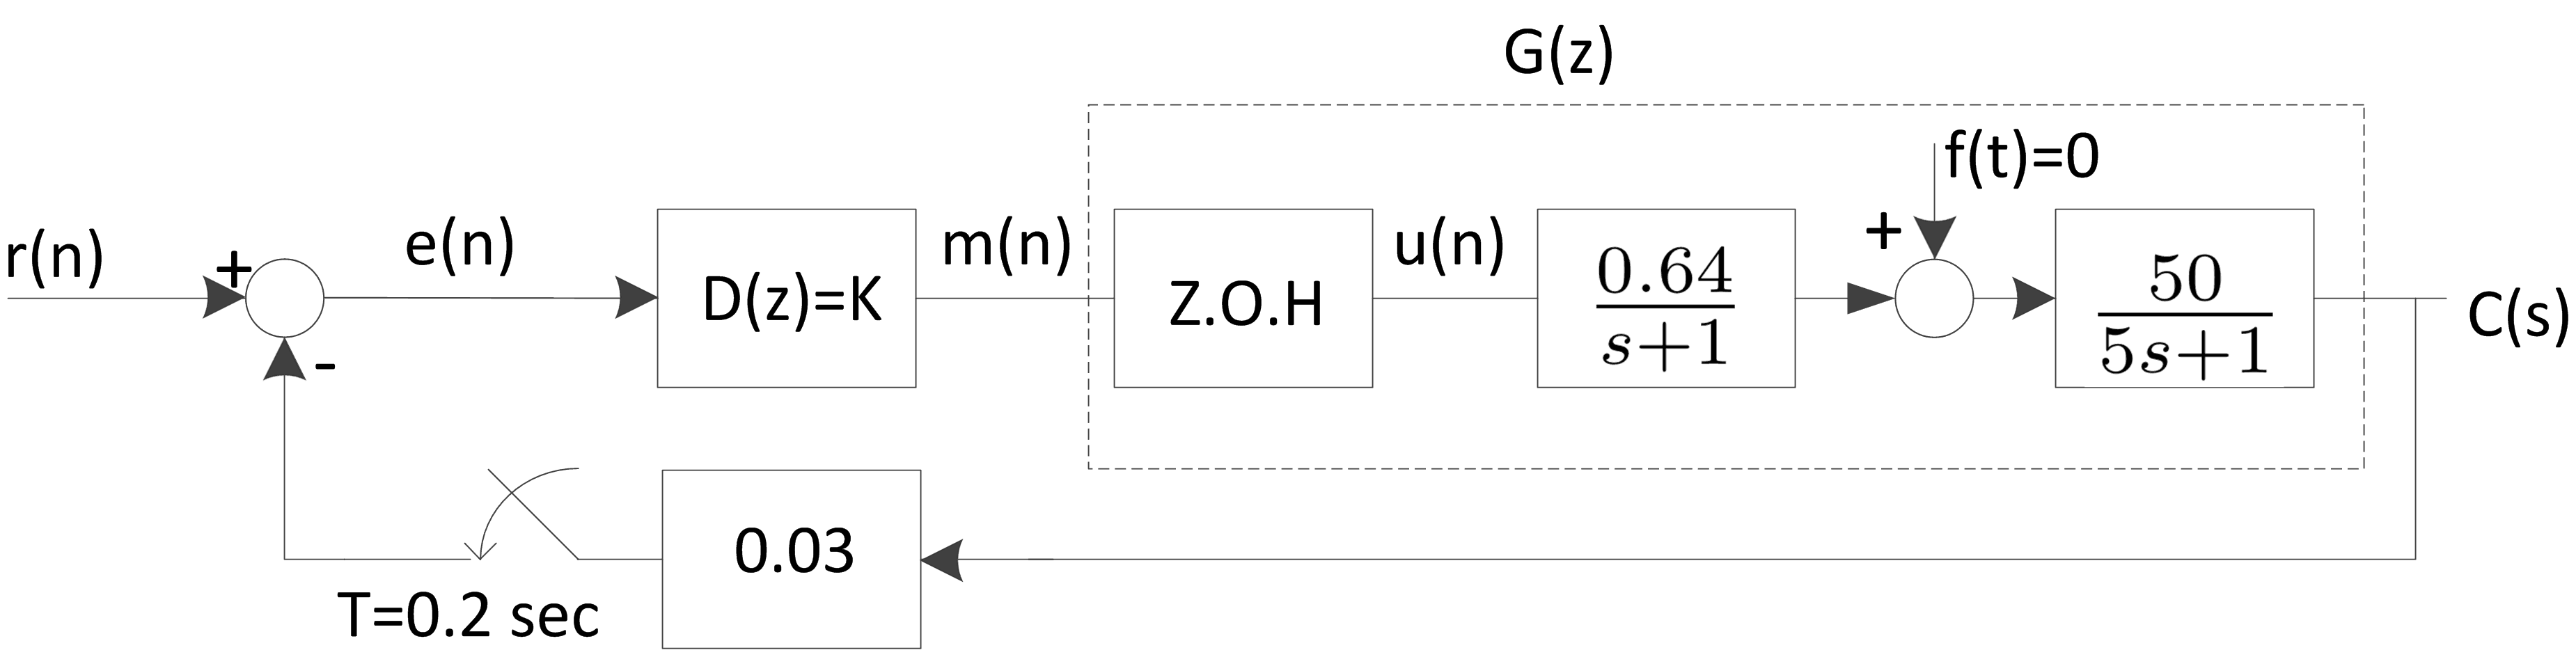
\includegraphics[width=.75\linewidth]{./Figures/example1_diag.png} \vspace{.05in}

$G(z) = (1-z^{-1})\Z\left[\frac{6.4}{s(s+1)(s+0.2)}\right] = \frac{0.16z+0.064}{z^2-1.78z+0.78}$ \\ \vspace{.05in}
Closed-loop transfer function, \\ \vspace{.05in}
$T(z) = \frac{C(z)}{R(z)}= \frac{KG(z)}{1+0.03KG(z)}$
}

%----------- slide --------------------------------------------------%
\frame
{
%\vspace{-.2in}
\normalsize

\frametitle{Jury's Stability Test-Cont.}

Thus, the CE of the closed-loop system, \\ \vspace{.05in}

$\varrho (z) = 1+0.03KG(z) = z^2-1.78z+0.78+0.03K(0.16z+0.064)=0$ \\
or,\\

$\varrho(z) = z^2-(1.78-0.0048K)z+(0.78+0.0019K) = 0$ \\ \vspace{.05in}
For stability,  \\ \vspace{.05in}
\begin{enumerate}
	\item $\varrho(1) >0 ~~\implies 0.007+0.0067K>0 \implies K>-1.04$\\
	\item $\varrho(-1)>0 \implies 3.57 - 0.0028K>0 \implies K<1.24 \times 10^3$
	\item $a_0<a_2~~~~\implies 0.78+0.0019K<1 \implies K<111$
\end{enumerate}

Therefore, the range of $K$ for stability is   $0<K<111$.  \\ \vspace{.05in}

\textcolor{red}{Example 2:} The CE of a digital control system is given by, \\ \vspace{.05in}

$\varrho(z) = z^3+(111.6 T^2+16.74T-3) z^2+(3-33.48T+1.395 \times 10^{-4}KT^3)z+(1.395 \times 10^{-4}KT^3+16.74T-111.6T^2-1) = 0$ \\ \vspace{.05in}

find the range of $T$ (sampling period) and gain $K$ for stability.\\



}

%----------- slide --------------------------------------------------%
\frame
{
%\vspace{-.2in}
\normalsize

\frametitle{Jury's Stability Test-Cont.}

\begin{enumerate}
	\item $\varrho(1)>0 \implies KT^3>0 \implies K>0$
	\item $\varrho(-1)<0 \implies -8+66.96 T<0 \implies T<0.12~sec $
	\item $|a_0|<a_3 \implies |1.395 \times 10^{-4}KT^3+16.74T-111.6T^2-1|<1 $
	\item $|b_0|>|b_2| \implies (1.395 \times 10^{-4}KT^3+16.74T-111.6T^2-1)^2-1> |(1.395 \times 10^{-4}KT^3+16.74T-111.6T^2-1)(111.6 T^2+16.74T-3)-(3-33.48T+1.395 \times 10^{-4}KT^3)| $
\end{enumerate}
The stable region can be identified by plotting. \\

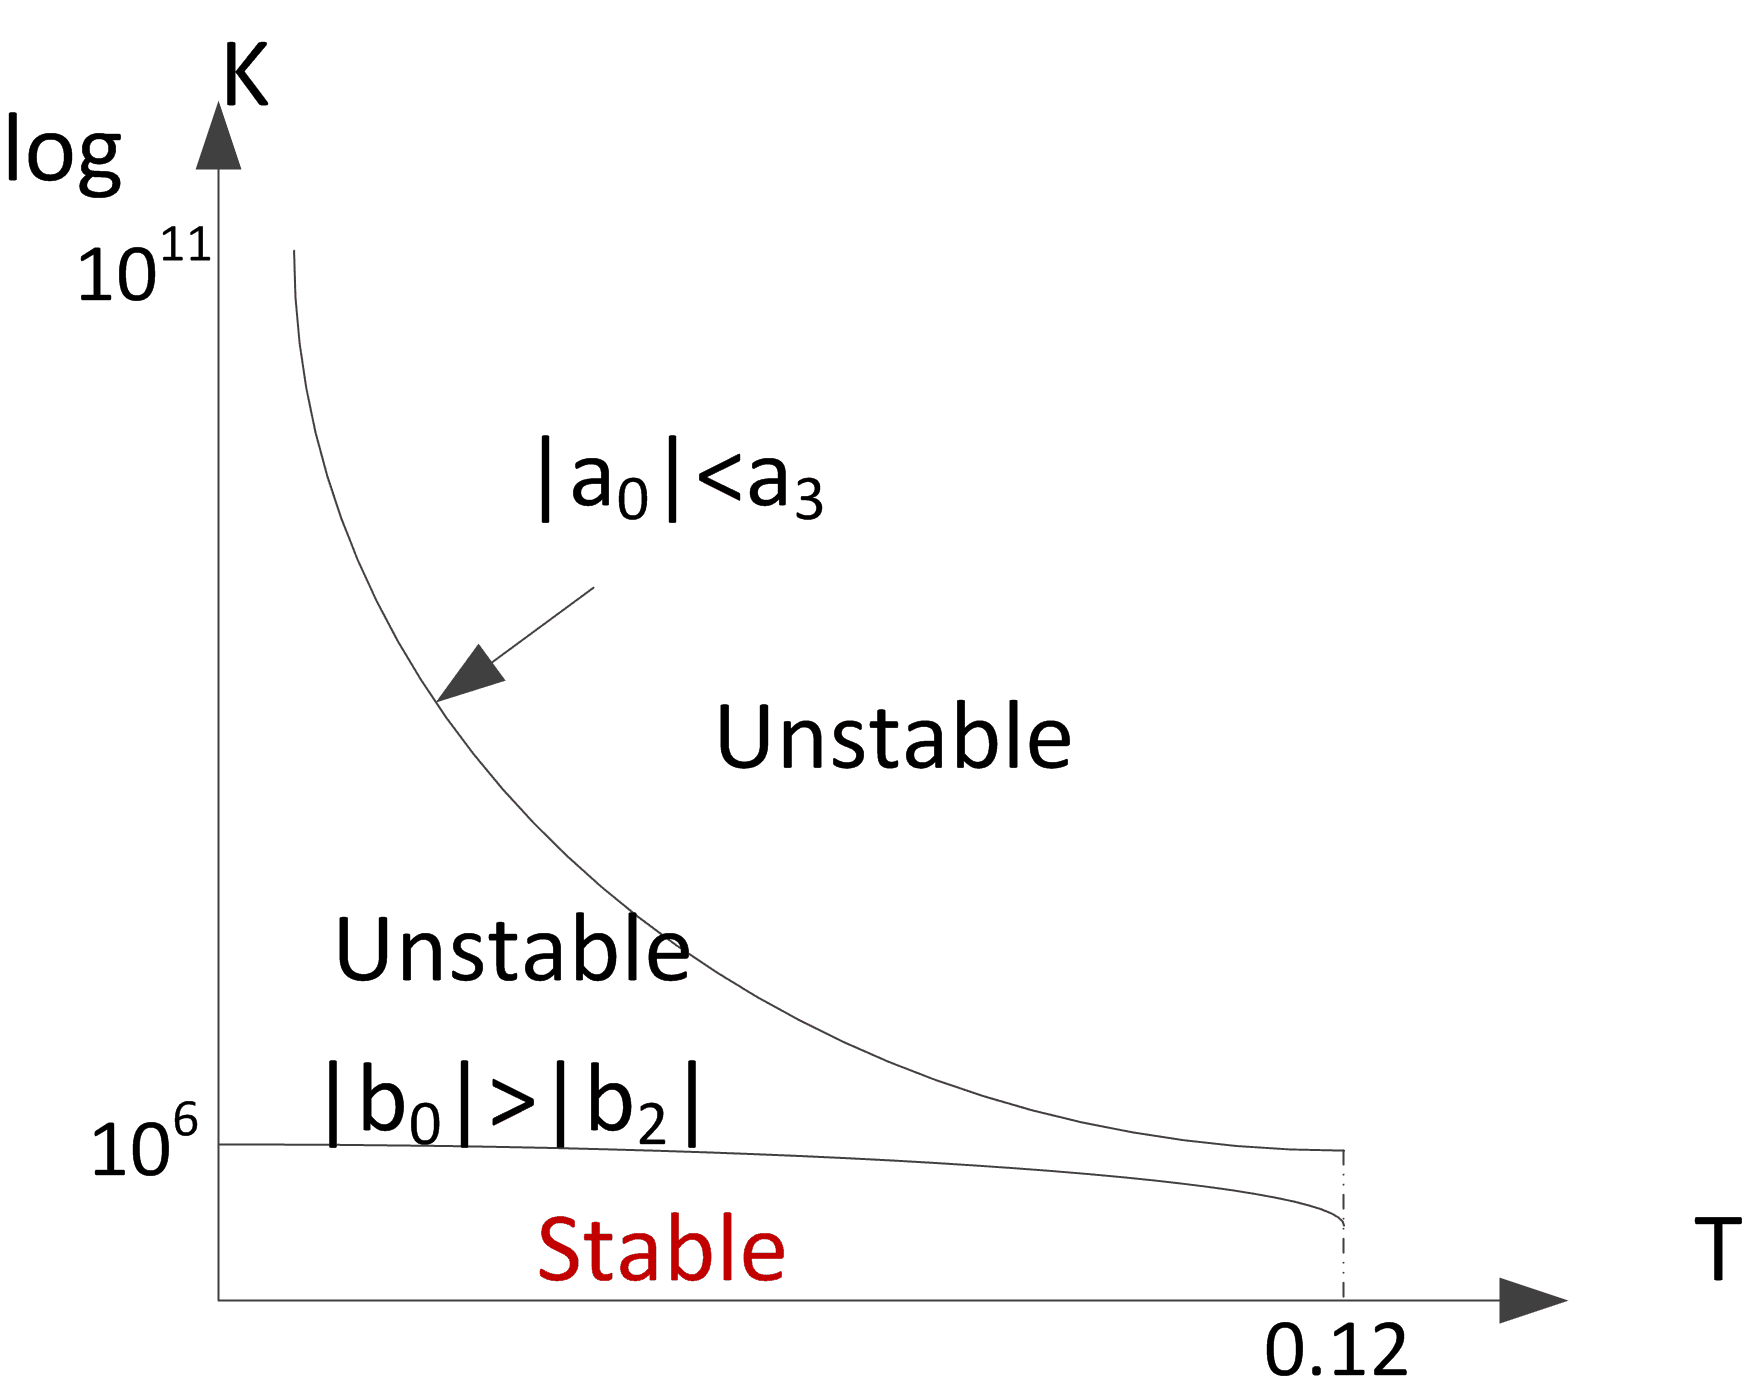
\includegraphics[width=.3\linewidth]{./Figures/rangekt.png} \vspace{.05in}

This example shows the utility of the Jury's test for design purposes as well.
}

%----------- slide --------------------------------------------------%
\frame
{
%\vspace{-.2in}
\normalsize

\frametitle{Jury's Stability Test-Cont. }

\textcolor{red}{Remark:}\\
When some or all elements of a row in Jury's table become zero, tabulation terminates. \\ \vspace{.05in}

\textcolor{red}{Remedy:}\\
Expand or contract the unit circle by $z \to (1\pm \epsilon)z$ where $\epsilon>0$\\
$z^N \to (1\pm \epsilon)^Nz^N$\\
But since $(1\pm \epsilon)^N \approx 1\pm N\epsilon$  we use $z^N \to (1\pm N \epsilon)z^N$. \\
i.e. we use $(1\pm N\epsilon)z^N$ instead of $z^N$ in table and proceed. \\ \vspace{.05in}

\textcolor{red}{Example:}\\ \vspace{.05in}
Let $\varrho(z) = z^3+z^2+z+1$\\

$\begin{array}{ccccc}
	Row&z^0&z^1&z^2&z^3\\
	1&1&1&1&1\\
	2&1&1&1&1\\
	3&0&0&0
\end{array}$\\
Substitute \\
$z^3 \to (1+3\epsilon)z^3$ , \hspace{0.1in}
$z^2 \to (1+2\epsilon)z^2$, \hspace{0.1in} and
$z \to (1+\epsilon)z$

}


%----------- slide --------------------------------------------------%
\frame
{
%\vspace{-.2in}
\normalsize

\frametitle{Jury's Stability Test-Cont. }

Then, Jury's table becomes \\ \vspace{.05in}

$\begin{array}{ccccc}
	Row&z^0&z^1&z^2&z^3\\
	1&1&1+\epsilon&1+2\epsilon&1+3\epsilon\\
	2&1+3\epsilon&1+2\epsilon&1+\epsilon&1\\
	3&-6\epsilon&-4\epsilon&-2\epsilon\\
	4&-2\epsilon&-4\epsilon&-6\epsilon
\end{array}$\\

\begin{enumerate}
	\item $\varrho(1)>0 \implies \varrho(1) = 4>0$
	\item $-\varrho(-1)>0 \implies \varrho(1) = 0$
	\item $|a_0|<|a_3| \implies 1<1+3\epsilon \implies \epsilon>0$
	\item $|b_0|>|b_2| \implies 6\epsilon>2\epsilon$
\end{enumerate}

Stable for $\epsilon>0$ and unstable for $\epsilon<0 \implies $ poles must be on the unit circle.

}


\section{Digital Filter Design}
%----------- slide --------------------------------------------------%
\frame
{
%\vspace{-.2in}
\normalsize


%\renewcommand{\theenumii}{\roman{enumi}}
%\renewcommand{\theenumi}{\alph{enumi}}

\frametitle{Design of Digital Filters}

Comprises of 4 general steps:\\

\begin{enumerate}
	\item \textcolor{blue}{Approximation:} Process of generating a transfer function satisfying a set of desired specs (frequency domain).
	\item \textcolor{blue}{Realization:} Process of converting a transfer function into a filter structure.
	\item \textcolor{blue}{Quantization effects:} Process of studying finite word length effects in digital systems.

		\begin{enumerate}[i]
			\item Input Quantization (at A/D).
			\item Coefficient Quantization  (at multipliers).
			\item Product Quantization  (output of multipliers).
		\end{enumerate}
	\item \textcolor{blue}{Implementation:} Process of implementing the designed filter either in
		\begin{enumerate}[i]
			\item Software, or
			\item Hardware.
		\end{enumerate}
\end{enumerate}




}

%----------- slide --------------------------------------------------%
\frame
{
%\vspace{-.2in}
\normalsize
%\renewcommand{\theenumi}{\alph{enumi}}
\frametitle{Approximation}

\textcolor{blue}{1. Approximation Methods for Recursive or IIR Digital Filters} \\
Consider a recursive digital filter described by difference equation (or transfer function):\\
$y(n) = \sum\limits_{i=0}^M b_i x(n-i) - \sum\limits_{j=1}^N a_j y(n-j)$\\
$x(n)$: input,~~$y(n)$ output,~~$N$: order,~~$a_j's, b_i's$: filter coefficients\\ \vspace{.1in}
\textcolor{red}{Advantages of IIR filters:} \\
\begin{enumerate}
	\item Low order (small $N$) gives sharper cutoff frequencies than FIR filters of the same order.
	\item Can be implemented easily in time-domain (recursive).
\end{enumerate}
\textcolor{red}{Disadvantages:}\\
\begin{enumerate}
	\item Nonlinear phase
	\item Stability issues 
	\item Quantization issues (limit-cycle oscillations)
\end{enumerate}


}

%----------- slide --------------------------------------------------%
\frame
{
%\vspace{-.2in}
\normalsize
%\renewcommand{\theenumi}{\alph{enumi}}
\frametitle{Approximation Methods}

\textcolor{red}{Indirect Methods:} Based on the design of analog prototype. \\ \vspace{.1in}

\textbf{Idea:}  Start with the design of an analog filter, $H_A(s)$, and map it to a digital transfer function, $H_D(z)$, i.e. $H_A(s) \to H_D(z)$ using an appropriate mapping:  \\ \vspace{.1in}
\begin{enumerate}
	\item Impulse Invariant \checkmark
	\item Bilinear $z$-Mapping \checkmark
	\item Matched $z$-Transform
\end{enumerate}


\textcolor{red}{Direct Methods:} Based on using optimization packages: \\
\begin{enumerate}
	\item Linear programming.
	\item Non-linear programming.
\end{enumerate}



}

%----------- slide --------------------------------------------------%
\frame
{
\vspace{-.2in}
\normalsize
%\renewcommand{\theenumi}{\alph{enumi}}
\frametitle{Indirect Method}

\textcolor{red}{Conditions for Mapping}\\
\begin{enumerate}
	\item Should preserve all essential \\characteristics of analog filter \\(BW, PB loss, SB loss).
	\item A stable analog filter should be \\mapped to a stable digital filter.
	\item The transfer function $H_D(z)$ \\should be rational and proper \\with real coefficients.
\end{enumerate}

$\omega_c:$ Cutoff frequency\\
$\omega_r:$  Lower stopband frequency\\
$\delta_1:$  Passband error\\
$\delta_2:$ Stopband error\\
\vspace{-2.1in}
\hspace{2.2in}
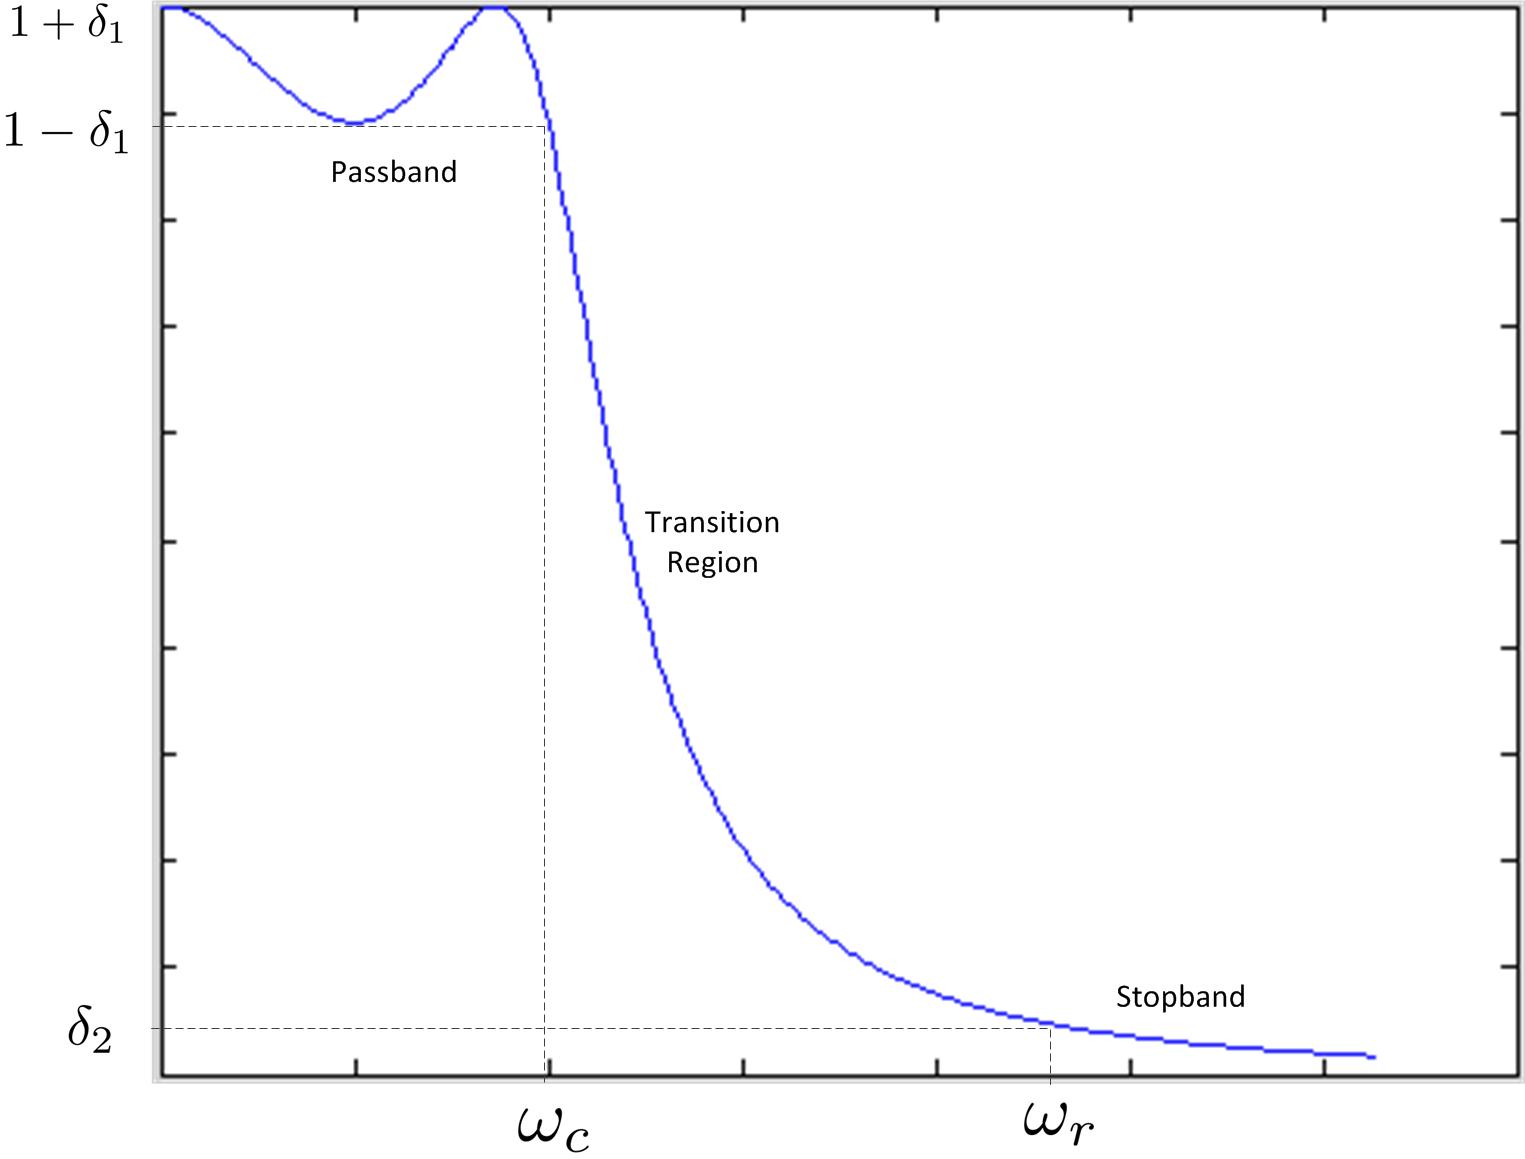
\includegraphics[width=.5\linewidth]{./Figures/lowpass_plot.png}

}

%----------- slide --------------------------------------------------%
\frame
{
%\vspace{-.2in}
\normalsize
%\renewcommand{\theenumi}{\alph{enumi}}
\frametitle{Review of Analog Filters-Preliminaries}
Recall:  $H_A(s) = \frac{Y(s)}{U(s)} = \int\limits_{0}^\infty h(t) e^{-st}dt$ \\ \vspace{.1in}
Define \textit{Magnitude-Squared Function}:\\ \vspace{.05in}
	 $A(-s^2) = H_A(s)H_A(-s)$ (Spectral Factorization)\\ \vspace{.05in}
Alternatively by letting $s=j\omega$ \\ \vspace{.05in}
$A(\omega^2) = H_A(j\omega)H_A(-j\omega) = H_A(j\omega)H^*_A(j\omega)=  |H_A(j\omega)|^2$\\ \vspace{.2in}

\textcolor{blue}{Properties of $A(-s^2)$:}\\

\begin{enumerate}
\item Even with real coefficients.
\item Complex poles and zeros of $A(-s^2)$ occur in quadruples i.e. if $p_i$ is a pole/zero then $-p_i$, $p^*_i$, and $-p^*_i$ are also poles/zeros. 
\end{enumerate}

\textcolor{red}{\textbf{Goal:}} Given $A(-s^2)$ (or $A(\omega^2)$), $H_A(s)$ should be chosen such that it contains all the poles and zeros of $A(-s^2)$ that lie in
the LH of the $s$-plane (spectral factorization). 


}

%----------- slide --------------------------------------------------%
\frame
{
%\vspace{-.2in}
\normalsize
%\renewcommand{\theenumi}{\alph{enumi}}
\frametitle{Review of Analog Filters-Preliminaries}
\textcolor{red}{Example:}\\
Given $A(\omega^2) = \frac{2+\omega^2}{1+\omega^4}$, determine $H_A(s)$. \\ \vspace{0.1in}

$A(-s^2) = \frac{2-s^2}{1+s^4} = \frac{(\sqrt{2}-s)(\sqrt{2}+s)}{(s+\alpha)(s+\alpha^*)(s-\alpha)(s+\alpha^*)} = H_A(s)H_A(-s)$\\
$\alpha = \frac{1+j}{\sqrt{2}}$\\
$H_A(s) = \frac{s+\sqrt{2}}{(s+\alpha)(s+\alpha^*)}$\\ \vspace{.1in}
i.e. $H_A(s)$ captures all poles/zeros that are in LH of $s$-plane.

}



\end{document}

